\documentclass{beamer}

\usepackage{amsmath}

\usetheme{AnnArbor}
\usecolortheme{crane}
\usefonttheme[onlymath]{serif}

\title{Deep Learning - Foundations and Concepts}
\subtitle{Chapter 10. Convolutional Networks}
\author{nonlineark@github}
\date{\today}

\begin{document}

\begin{frame}
    \titlepage
\end{frame}

\begin{frame}
    \frametitle{Outline}
    \tableofcontents
\end{frame}

\section{Computer Vision}

\begin{frame}
    \frametitle{Computer vision}
    \begin{itemize}
        \item Computer vision was one of the first fields to be transformed by the deep learning revolution, predominantly thanks to the CNN architecture.
        \item Recently alternative architectures based on transformers have become competitive with convolutional networks in some applications.
        \item Some applications for machine learning in computer vision: Classification, detection, segmentation, caption generation, synthesis, inpainting, style transfer, super-resolution, depth prediction, scene reconstruction.
    \end{itemize}
\end{frame}

\begin{frame}
    \frametitle{Image data}
    \begin{itemize}
        \item The structure of an image:
        \begin{itemize}
            \item An image comprises a rectangular array of pixels.
            \item Each pixel has either a grey-scale intensity or a triplet of red, green and blue channels each with its own intensity value.
        \end{itemize}
        \item Challenges of applying neural networks to image data:
        \begin{itemize}
            \item Images generally have a high dimensionality.
            \item Image data is highly structured.
        \end{itemize}
        \item Local correlations can be used to encode strong inductive biases into a neural network, leading to models with far fewer parameters and with much better generalization accuracy.
    \end{itemize}
\end{frame}

\section{Convolutional Filters}

\begin{frame}
    \frametitle{Inductive biases}
    To exploit the two-dimensional structure of image data to create inductive biases, we can use four interrelated concepts:
    \begin{itemize}
        \item Hierarchy.
        \item Locality.
        \item Equivariance.
        \item Invariance.
    \end{itemize}
\end{frame}

\begin{frame}
    \frametitle{Feature detectors}
    Let's restrict our attention to grey-scale images first. Consider a single unit in the first layer of a neural network:
    \begin{itemize}
        \item It takes as input just the pixel values from a small rectangular region, or patch, from the image. This patch is referred to as the receptive field of that unit.
        \item The output of this unit is given by the usual functional form comprising a weighted linear combinations of the input values, which is subsequently transformed using a nonlinear activation function: $z=\mathrm{ReLU}(w^{T}x+w_{0})$.
        \item The weights themselves form a small two-dimensional grid known as a filter, sometimes also called a kernel.
        \item The unit acts as a feature detector that signals when it finds a sufficiently good match to its kernel (basic properties of inner product).
    \end{itemize}
\end{frame}

\begin{frame}
    \frametitle{Feature detectors}
    \begin{figure}
        \caption{A single unit in the first layer of a neural network}
        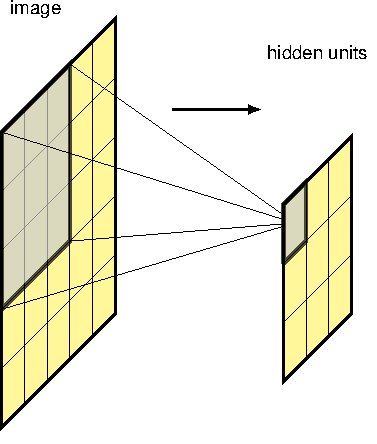
\includegraphics[height=0.7\textheight]{Figure_1_a.pdf}
    \end{figure}
\end{frame}

\begin{frame}
    \frametitle{Translation equivariance}
    \begin{itemize}
        \item To generalize what our neural network has learned in one location to all possible locations in the image, we can simply replicate the same hidden-unit weight values at multiple locations across the image.
        \item The units of the hidden layer form a feature map in which all the units share the same weights.
    \end{itemize}
    For an image $I$ with pixel intensities $I(j,k)$, and a filter $K$ with pixel values $K(l,m)$, the feature map $C$ has activation values given by:
    \begin{equation*}
        C(j,k)=\sum_{l}\sum_{m}I(j+l,k+m)K(l,m)
    \end{equation*}
    where we have omitted the nonlinear activation function for clarity. This is an example of a convolution and is sometimes expressed as $C=I*K$.
\end{frame}

\begin{frame}
    \frametitle{Translation equivariance}
    \begin{figure}
        \caption{A $3\times{}3$ image convolved with a $2\times{}2$ filter}
        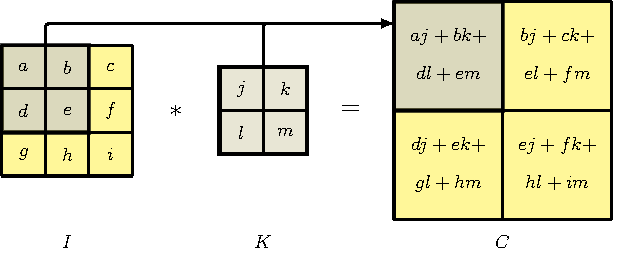
\includegraphics{Figure_3.pdf}
    \end{figure}
\end{frame}

\begin{frame}
    \frametitle{Translation equivariance}
    Comparing this convolutional structure with a standard fully connected network, we see several advantages:
    \begin{itemize}
        \item The connections are sparse, leading to far fewer weights even with large images.
        \item The weight values are shared, greatly reducing the number of independent parameters and consequently reducing the required size of the training set.
        \item The same network can be applied to images of different sizes without the need for retraining.
        \item Convolutions can be implemented very efficiently by exploiting the massive parallelism of GPUs.
    \end{itemize}
\end{frame}

\begin{frame}
    \frametitle{Padding}
    Consider an image of dimensionality $J\times{}K$ and a kernal of dimensionality $M\times{}M$:
    \begin{itemize}
        \item The feature map is of dimensionality $(J-M+1)\times(K-M+1)$, which is smaller than the original image.
        \item We can pad the original image with additional pixels around the outside. If we pad with $P$ pixels then the output map has dimensionality $(J+2P-M+1)\times(K+2P-M+1)$:
        \begin{itemize}
            \item If $P=0$, this is called a valid convolution.
            \item If $P=\frac{M-1}{2}$, this is called a same convolution.
        \end{itemize}
        \item Padding values are typically set to zero, after first subtracting the mean from each image so that zero represents the average value of the pixel intensity.
    \end{itemize}
\end{frame}

\begin{frame}
    \frametitle{Strided convolutions}
    Sometimes we wish to use feature maps that are significantly smaller than the original image to provide flexibility in the design of convolutional network architectures. One way to achieve this is to use strided convolutions in which, the filter is moved in larger steps of size $S$, called the stride. The feature map will have dimensionality:
    \begin{equation*}
        (\lfloor\frac{J+2P-M}{S}\rfloor+1)\times(\lfloor\frac{K+2P-M}{S}\rfloor+1)
    \end{equation*}
\end{frame}

\begin{frame}
    \frametitle{Multi-dimensional convolutions}
    We can easily extend convolutions to cover multiple channels by extending the dimensionality of the filter:
    \begin{itemize}
        \item An image with $J\times{}K$ pixels and $C$ channels will be described by a tensor of dimensionality $J\times{}K\times{}C$.
        \item We can introduce a filter described by a tensor of dimensionality $M\times{}M\times{}C$.
    \end{itemize}
\end{frame}

\begin{frame}
    \frametitle{Multi-dimensional convolutions}
    \begin{figure}
        \caption{A multi-dimensional filter}
        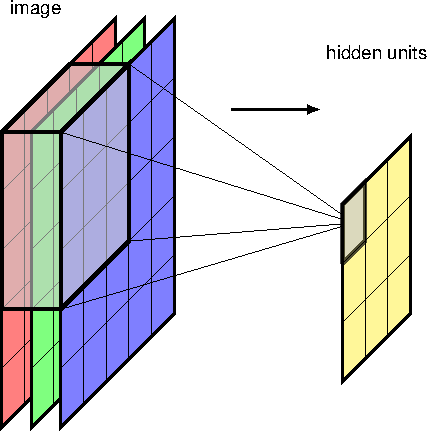
\includegraphics[height=0.7\textheight]{Figure_6_a.pdf}
    \end{figure}
\end{frame}

\begin{frame}
    \frametitle{Multi-dimensional convolutions}
    To build more flexible models, we simply include multiple filters, in which each filter has its own independent set of parameters giving rise to its own independent feature map:
    \begin{itemize}
        \item We again refer to these separate feature maps as channels.
        \item The filter tensor now has dimensionality $M\times{}M\times{}C\times{}C_{\textrm{OUT}}$ where $C$ is the number of input channels and $C_{\textrm{OUT}}$ is the number of output channels.
        \item Each output channel will have its own associated bias parameter, so the total number of parameters will be $(M^{2}C+1)C_{\textrm{OUT}}$.
    \end{itemize}
\end{frame}

\begin{frame}
    \frametitle{Pooling}
    Small changes in the relative locations do not affect the classification, and we want to be invariant to such small translations of individual features. This can be achieved using pooling:
    \begin{itemize}
        \item A pooling layer is similar to a convolutional layer:
        \begin{itemize}
            \item Each unit takes input from a receptive field in the previous feature map layer.
            \item There is a choice of filter size and of stride length.
        \end{itemize}
        \item The difference is that the output of a pooling unit is a simple, fixed function of its inputs:
        \begin{itemize}
            \item Max-pooling.
            \item Average pooling.
        \end{itemize}
    \end{itemize}
\end{frame}

\begin{frame}
    \frametitle{Pooling}
    \begin{figure}
        \caption{Illustration of max-pooling}
        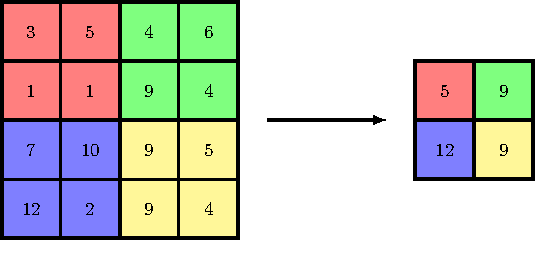
\includegraphics{Figure_8.pdf}
    \end{figure}
\end{frame}

\begin{frame}
    \frametitle{Multilayer convolutions}
    \begin{itemize}
        \item To allow the network to discover and represent hierarchical structure in the data, we extend the architecture by considering multiple layers.
        \item Each convolutional layer is described by a filter tensor of dimensionality $M\times{}M\times{}C_{\textrm{IN}}\times{}C_{\textrm{OUT}}$ in which the number of independent weight and bias parameters is $(M^{2}C_{\textrm{IN}}+1)C_{\textrm{OUT}}$.
        \item Each such convolutional layer can optionally be followed by a pooling layer.
        \item In many applications (e.g., classification tasks), the output units need to combine information from across the whole of the input image. This is typically achieved by introducing one or two standard fully connected layers as the final stages of the network.
    \end{itemize}
\end{frame}

\begin{frame}
    \frametitle{Example network architectures}
    \begin{figure}
        \caption{The architecture of a convolutional network called VGG-16}
        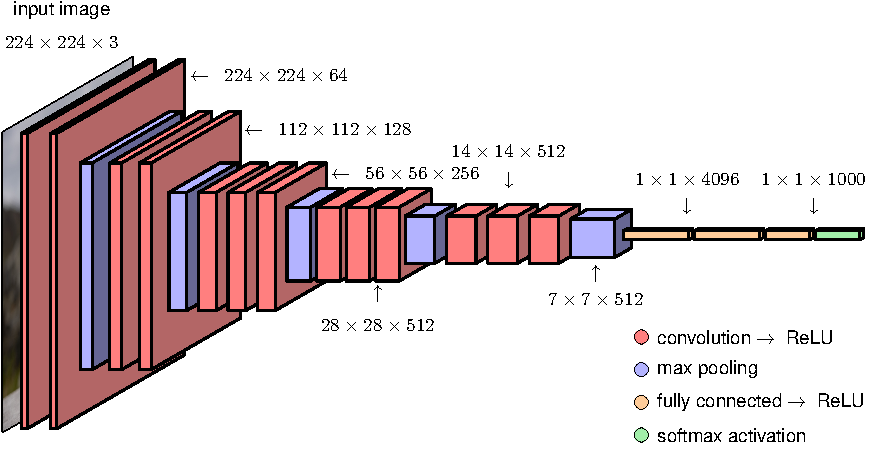
\includegraphics[width=0.8\textwidth]{Figure_10.pdf}
    \end{figure}
\end{frame}

\end{document}